\documentclass{article}
\usepackage[a4paper, tmargin=1in, bmargin=1in]{geometry}
\usepackage[utf8]{inputenc}
\usepackage{graphicx}
\usepackage[justification=centering]{caption}

% \usepackage{parskip}
\usepackage{pdflscape}
\usepackage{listings}
\usepackage{hyperref}
\usepackage{caption}
\usepackage{subcaption}
\usepackage{float}
\usepackage{enumerate}
\usepackage{amsmath}

\setlength{\parindent}{0pt}

\title{CS 754 : Advanced Image Processing\\
Assignment 5}
\author{Meet Udeshi - 14D070007\\
  Arka Sadhu - 140070011\\
}
\date{\today}

\newcommand{\lone}[1]{
  ||#1||_{l_1}
}
\newcommand{\ltwo}[1]{
  ||#1||_{l_2}
}
\newcommand{\linf}[1]{
  ||#1||_{l_\infty}
}
\newcommand{\dbint}{
  \int_{\infty}^{\infty}\int_{\infty}^{\infty}
}

\begin{document}
\maketitle
\section*{Q1}

\textbf{Mutual Coherence:}

\[ \mu = 0.996815820660457 \]

\textbf{Histogram of Coherence Values:}

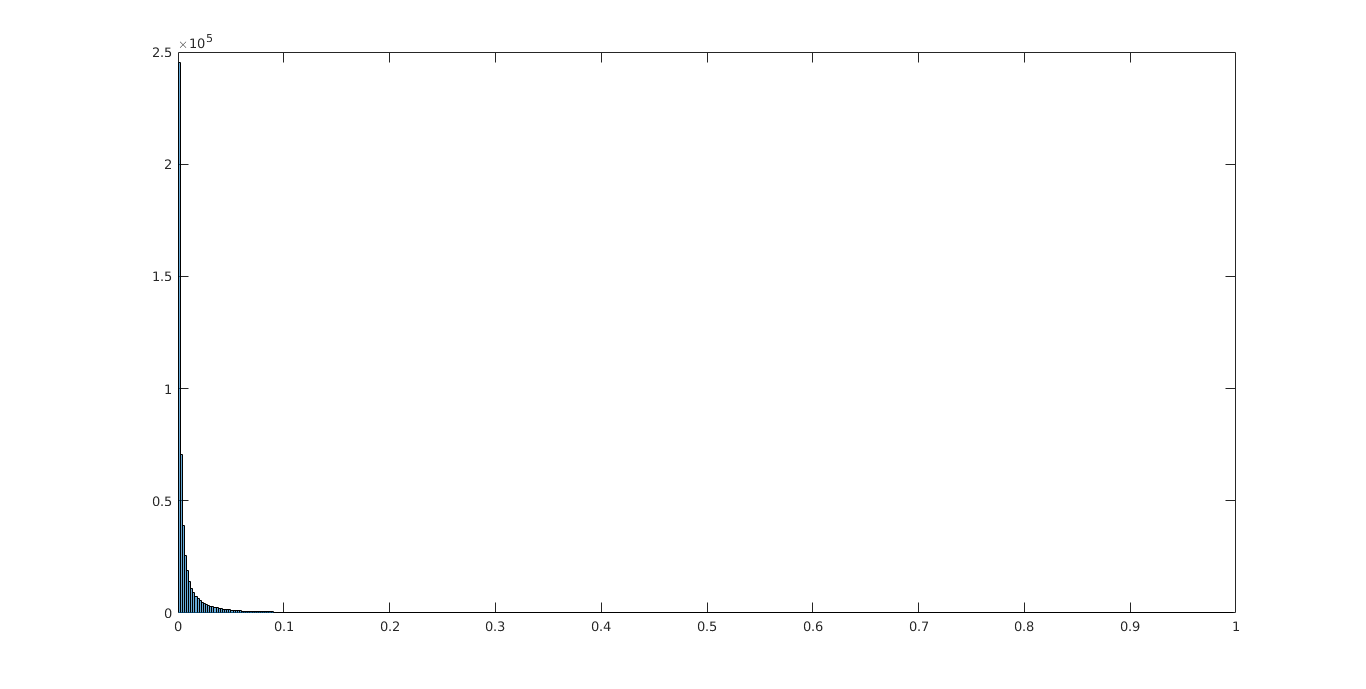
\includegraphics[scale=0.5]{coherence_hist.png}

\section*{Q2}
\subsection*{A2.1}
Need to show Shift Theorem:
\begin{equation}
  \label{eq:1}
R(g(x-x_0,y-y_0)(\rho,\theta) = R(g(x,y))(\rho - x_0cos(\theta) - y_0sin(\theta),\theta)  
\end{equation}

Let $h(x,y) = g(x-x_0,y-y_0)$
$$R(h(x,y))(\rho,\theta) = \dbint h(x,y)\delta(xcos(\theta) + ysin(\theta) - \rho)dxdy$$
$$R(h(x,y))(\rho,\theta) = \dbint g(x-x_0,y-y_0)\delta(xcos(\theta) + ysin(\theta) - \rho)dxdy$$
Put $x_1 = x - x_0$ and $y_1 = y - y_0$
$$R(h(x,y))(\rho,\theta) = \dbint g(x_1,y_1)\delta((x_1 + x_0)cos(\theta) + (y_1 + y_0)sin(\theta) - \rho) dxdy$$
$$R(h(x,y))(\rho,\theta) = \dbint g(x_1,y_1)\delta(x_1cos(\theta) + y_1sin(\theta) - (\rho - x_0cos(\theta) - y_0sin(\theta)) dx_1dy_1 = R(g(x,y)(\rho_1,\theta)$$
where $\rho_1 = \rho - x_0cos(\theta) - y_0sin(\theta)$\\
Therefore
$$R(h(x,y))(\rho,\theta) = R(g(x-x_0,y-y_0))(\rho,\theta) = R(g(x,y))(\rho_1,\theta)$$
Hence Proved

\subsection*{A2.2}
Need to show Rotation Theorem:
Let $g^{'}(r,\psi) = g(r,\psi - \psi_0). $
\begin{equation}
  \label{eq:2}
  R(g^{'})(\rho,\theta) = R(g)(\rho,\psi_0 - \theta)
\end{equation}
$$R(g^{'}(r,\psi))(\rho,\theta) = \dbint g^{'}(r,\psi)\delta(\rho - rcos(\psi - \theta))|r|drd\psi$$
$$R(g^{'}(r,\psi))(\rho,\theta) = \dbint g(r,\psi - \psi_0)\delta(\rho - rcos(\psi - \theta))|r|drd\psi$$
Put $\psi_1 = \psi - \psi_0$
$$R(g^{'}(r,\psi))(\rho,\theta) = \dbint g(r,\psi_1)\delta(\rho - rcos(\psi_1 + \psi_0 - \theta)|r|drd\psi_1$$
$$R(g^{'}(r,\psi))(\rho,\theta) = R(g(r,\psi))(\rho,\psi_0 - \theta)$$

\subsection*{A2.3}
Need to show Convolution Theorem:
Let $$h(x,y) = \dbint f(x_1,y_1)g(x - x_1,y - y_1)dx_1dy_1$$
\begin{equation}
  \label{eq:3}
  Rh = Rf * Rg
\end{equation}
$$Rh = \dbint\dbint f(x_1,y_1)g(x-x_1,y-y_1)\delta(\rho - xcos(\theta) - ysin(\theta))dx_1dy_1dxdy$$
$$Rh = \dbint \dbint R(g)(\rho - x_1cos(\theta) - y_1sin(\theta),\theta) dx_1dy_1$$

$$Rh = \dbint \int_{\infty}^{\infty}f(x_1,y_1)R(g(\rho-\rho_1,\theta)\delta(\rho_1 - x_1cos(\theta) - y_1sin(\theta))dx_1dy_1d\rho_1$$
$$Rh = \int_{\infty}^{\infty}R(f)(\rho_1,\theta)R(g))(\rho - \rho_1,\theta)d\rho_1$$
$$Rh = Rf * Rg$$
\end{document}
